\documentclass{article}
%%%%%%%%%%%%%%%%%%%%%%%%%%%%%%%%%%%%%%%%%%%%%%%%%%%%%%%%%%%%
\usepackage{graphicx} % Required for inserting images
\usepackage{neurips_2023}
%%%%%%%%%%%%%%%%%%%%%%%%%%%%%%%%%%%%%%%%%%%%%%%%%%%%%%%%%%%%
\usepackage[utf8]{inputenc} % allow utf-8 input
\usepackage[T1]{fontenc}    % use 8-bit T1 fonts
\usepackage{hyperref}       % hyperlinks
\usepackage{url}            % simple URL typesetting
\usepackage{booktabs}       % professional-quality tables
\usepackage{amsfonts}       % blackboard math symbols
\usepackage{nicefrac}       % compact symbols for 1/2, etc.
\usepackage{microtype}      % microtypography
\usepackage{xcolor}         % colors
\usepackage{kotex}

\usepackage{indentfirst}

\setlength{\parindent}{0.1in} % 들여쓰기 길이 설정
\setlength{\parskip}{1mm} % 문단 간의 간격 조절
%%%%%%%%%%%%%%%%%%%%%%%%%%%%%%%%%%%%%%%%%%%%%%%%%%%%%%%%%%%%



\title{역할기반 멀티모달 퓨전을 활용한\\ 뉴스기사 분류}
\author{윤이상}
\date{2023년 10월}

\begin{document}

\maketitle

\begin{abstract}
정보의 전달은 텍스트뿐만 아니라, 사진, 영상, 음성 등의 다양한 형태로 이루어진다. 이에 데이터 분석에서 멀티 모달 모형의 활용이 주목을 받고 있다. 본 논문에서는 인터넷 신문의 텍스트 데이터와 이미지 데이터를 모두 분석에 반영하는 멀티 모달 모형 RoBaMF를 제안한다. RoBaMF에서는 이미지와 주석의 상호작용을 반영하고자 feature-fusion을 사용한 모형을 포함한다. 또한, 텍스트와 이미지의 단일 모형도 함께 고려하는 앙상블 방법론을 고려한다. 연구 결과, RoBaMF는 기사(article)-이미지 복합 모형보다 향상된 accuracy를 보이지 못했다.
\end{abstract}

\section{Introduction}
인터넷 뉴스는 제목과 본문, 사진과 사진에 대한 주석으로 이루어져 있다. 카테고리를 분류하기 위해, 텍스트 정보와 이미지 정보를 모두 분석에 포함하는 멀티 모달 모형을 고려하는 것이 합리적이다. 더불어서 주석은 이미지를 자세히 설명해주는 역할을 하기 때문에, 사진과 주석은 강한 연관성이 있다. 본 연구에서는 뉴스 기사 카테고리 분류 문제에서 주석의 역할을 분석에 포함하는 RoBaMF 모형을 제안한다. 이 모형은 이미지와 주석의 상호작용을 반영하기 위해, feature-fusion을 사용한 기본 분류기를 포함한다. 더불어 신문에서 중요한 역할을 하는 기사 텍스트 (article)와 이미지의 고유한 정보를 반영하기 위해, 각 대상에 대한 기본 분류기를 포함하였다. 세 기본 분류기에 앙상블 방법을 적용하여 결과를 산출하였다.

\section{Related Work}
\subsection{Text 기반 뉴스 분류 선행 연구}
Suh Y, Yu J, Mo J, Song L. (2017)은 네이버 기사들에 대해 Logistic Regression(LR), SVM, Naïve Bayes, KNN 등을 이용한 카테고리를 분류를 수행하였다\cite{suh2017comparison}.
Yoon (2014)는 단어 임베딩 행렬을 입력값으로 하는 CNN 문서 분류 모형 TextCNN을 제시하였다\cite{kim2014convolutional}.
Jang B, Kim I, Kim JW (2019)는 Word2Vec과 CNN을 이용한 트윗, 뉴스 분류를 수행하였으며, Word2Vec이 단어간 의미 관계 (semantic relationship)을 학습하여 더 나은 성능을 보인다는 것을 보였다\cite{jang2019word2vec}.
Nishant Rai, Deepika Kumar, Naman Kaushik, Chandan Raj, Ahad Ali (2022)는 BERT와 LSTM을 결합하여 가짜 뉴스분류를 수행하였다\cite{rai2022fake}.

\subsection{Feature Fusion}
feature fusion은 두 자료에서 추출한 정보를 하나로 융합하는 것을 말한다. 이는 이질적인 feature들을 하나의 벡터로 만드는 것을 뜻한다.
feature-fusion의 단순한 방법으로는 maximization, summation, concatenation이 있다.
Nicolas Audebert, Catherine Herold, Kuider Slimani, Cédric Vidal (2019) 에서는 이미지-텍스트 멀티모달 분류 문제에서concatenation 방법을 사용하였다\cite{audebert2020multimodal}.
해당 논문에서는 summation 방법을 사용한 모형이 이미지만 사용한 모형(pure-image model)보다 성능이 저조하다고 밝혔으며, 이는 summation이 이미지와 텍스트 각각의 고유한 결정력(discriminating power)을 저해하기 때문이라고 추론했다.
복잡한 feature-fusion 방법으로 Jian Yang(2002)는 parallel feature fusion\cite{yang2003feature}을 제안하였으며, Yimian Dai(2021)는 attentional feature fusion\cite{dai2021attentional}을 제안하였다.


\subsection{앙상블 모델}
앙상블 방법론은 다수의 기본 모형들을 결합하여 예측의 정확도를 향상시키는 방법이다.
Yawen Xiao, Jun Wu, Zongli Lin, Xiadong Zhao(2017)은 딥러닝 기반 다중 모형 앙상블 방법론을 제시하여 우수한 결과를 보였다\cite{xiao2018deep}.
Silvia Corchs, Elisabetta Fersini \& Francesca (2019)에서는 이미지-텍스트 멀티모달 데이터에 대해 BMA(Bayesian Model Averaging) 앙상블 방법론을 적용한 감성 분석을 수행하였다\cite{corchs2019ensemble}.


\section{Methodology}
\subsection{Textual Features}
텍스트 데이터로부터 feature을 추출하는 것이 목적이므로, 제목(title)과 본문(body) 텍스트가 포함된다.
본 연구에서는 텍스트 feature 추출에 KoBERT를 사용한다.
KoBERT 모형은 한국어 위키와 뉴스에서 발췌한 문장을 학습한 자연어 처리 모형으로,
 /기존 BERT\cite{devlin2018bert}의 한국어 성능 한계 극복을 위해서 개발되었으며 뉴스 등으로 수집한 한국어 문장으로 이루어진 corpus를 학습하였고 한국어 특유의 언어 변화의 특성을 반영하기 위하여 SentencePiece tokenizer를 적용하여 긴 문자열도 하나의 토큰으로 처리할 수 있게 해주며 기존대비 27%이상의 성능 향상을 보였다./
링 리듀스-기반 분산 학습 기술 설명 하기(종혁)/
다국어를 지원하는 MBERT에 비해 한국어 자연어 처리에 있어서 우수한 성능을 보인다.
실제로, 한국 이커머스 상품평 감성분석, 기업 관련 한국어 뉴스 감성분석에서 KoBERT는 MBERT보다 우수한 결과를 보였다.

\subsection{Visual features}
Fine-tune된 심층 CNN을 통해 추출된 visual feature들을 이용하는 것은, visual recognition task에서 우수한 기준선이 될 수 있다\cite{sharif2014cnn}.
이에 근거하여, 본 연구에서는 ImageNet으로 fine-tune 된 MobileNetV2를 이용하여 뉴스의 이미지로부터 심층 visual feature을 추출하였다.
MobileNetV2는 MobileNet의 후속 모형으로, inverted residual구조를 통해 모형의 크기와 연산량을 줄이면서 성능을 향상시켰다.
MobileNetV2는 병목 블록(bottleneck block)이 쌓인 구조이다. 각 병목 블록은 narrow pointwise convolution과 identity activation, 3 by 3 wide depthwise separable convolution과 ReLU activation, narrow pointwise convolution과 ReLU, 세 단계의 연산을 순차적으로 수행한다.
Ke Dong, Chenjie Zhou, Yihan Ruan, Yuzhi Li (2020)는 MobileNet V2로 이미지 분류를 수행하여 기존의 모형들보다 좋은 결과를 보였다\cite{dong2020mobilenetv2}.

\subsection{Feature fusion}
본 연구에서는 MobileNetV2를 이용하여 이미지 feature을 추출하고, KoBERT를 이용하여 주석의 feature을 추출한 뒤 이를 순방향 신경망 모형에 입력하였다. 그러기 위해, 두 feature 벡터를 열 방향으로 합쳐 한 개의 벡터로 만들었다.
이러한 feature-fusion을 concatenate 방법이라고 부르며, 다음과 같은 강점을 가지고 있다.
1. 정보 보존 : Concatenate는 특징 벡터를 단순히 연결하기 때문에, 합치고자 하는 두 feature 벡터의 크기와 특성을 고려할 필요가 없다. 이로써 각 도메인에서 추출한 특성이 완전히 유지되며 정보의 손실이 최소화된다. 따라서 각 도메인의 결정력을 보존해야 하는 멀티모달 데이터에 유리하다.
 
2. 유연성 : Concatenate는 feature을 추출하는 방법 (feature extractor)이 바뀌어도 영향을 받지 않는다. 예를 들어, 본 논문에서 이미지 feature 추출을 위해 고려하는 MobileNetV2를 ResNet과 같은 다른 CNN모형으로 대체할 수 있다.

\subsection{앙상블}
본 연구에서는 이미지와 주석의 상호작용을 고려할 뿐만 아니라, 뉴스의 주요 내용인 기사와 이미지의 고유한 정보를 함께 고려하고자 한다.
또한, 우리는 이미지와 주석의 상호작용이 뉴스 카테고리 분류 성능에 미치는 영향을 파악하고자 한다.
위 두가지를 모두 고려하기 위해, 최종 모형에 stacking 앙상블 방법론을 적용하였다.
 Stacking 앙상블 방법론은 기본 분류기(level 1 classifier)들의 예측확률을 메타 모형(level 2 classifier, meta learner)의 입력값으로 사용하는 방법이다. 메타 모형으로 의사결정나무 기반의 XGBoost를 사용하면 변수 중요도를 계산할 수 있다. 이를 통해 이미지-주석의 상호작용 모형이 분류에 미치는 영향을 변수 중요도를 통해 파악할 수 있다.
본 연구에서는 위 과정을 통해 만들어진 멀티 모달 분류 모형을 Role-Based Multimodal Fusion 모형, 이하 RoBaMF 모형이라고 한다. RoBaMF 모형의 전체적인 도식은 그림 1. 과 같다.


\begin{figure}[ht]
    \centering
    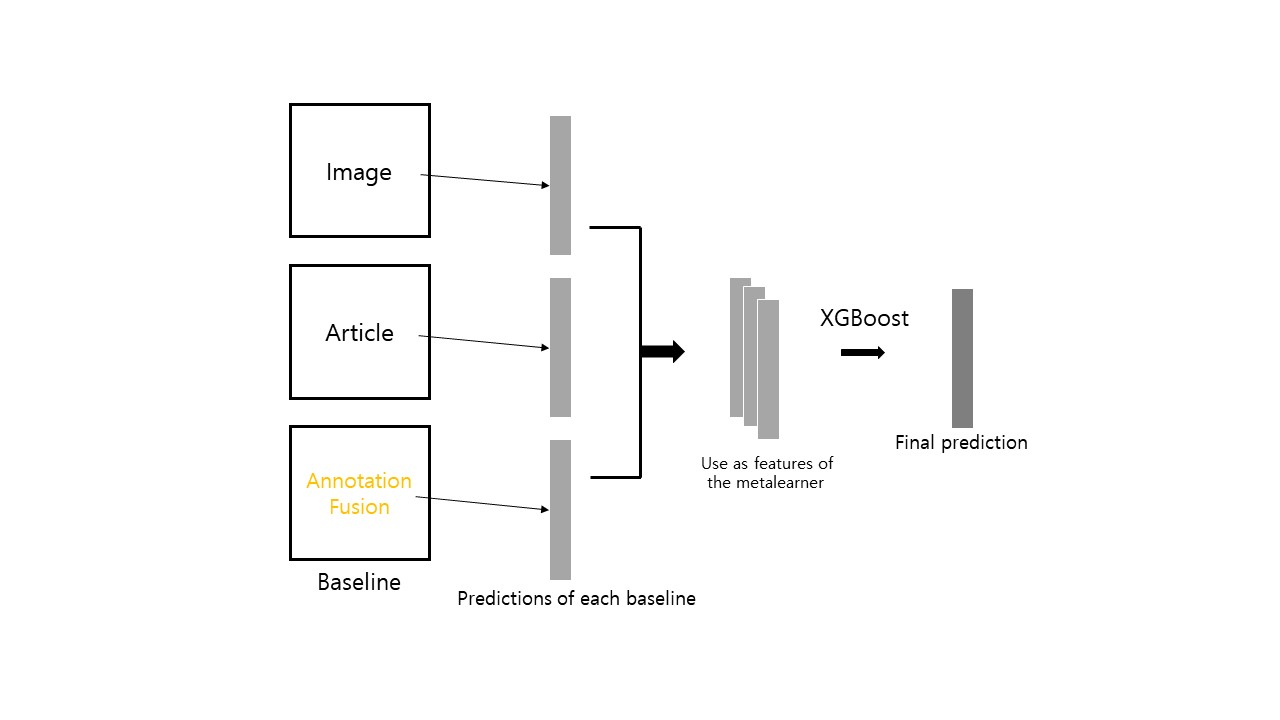
\includegraphics[width=\columnwidth]{ENG/fig.1.jpg}
    \caption{The overall pipeline of the RoBaMF model}
    \label{fig.1}
\end{figure}

\section{실험}
\subsection{데이터셋}
네이버 인터넷 뉴스는 정치, 경제, 사회, 생활/문화, IT/과학, 세계 등 6개의 주요 카테고리로 나누어져 있다. 이미지가 포함되지 않은 뉴스는 크롤링 대상에서 배제하였으며, 연구에 부합하지 않은 데이터를 포함한 뉴스는 크롤링 이후 가려내었다. 
하나의 기사에서 카테고리, 제목-본문(Article), 이미지(Image)-주석(Annotation) 쌍을 추출하였다.
총 12920개의 기사가 데이터셋에 포함되었다. 각 카테고리에서 1200개의 기사를 무작위로 추출하여 훈련 데이터로 사용하였으며, 나머지 기사들은 시험 데이터로 사용하였다.


\subsection{모델}
이 subsection에는 우리의 RoBaMF모형과 더불어 비교 대상 모형들의 구현 방식에 대해 기술하였다. 모든 모형은 PyTorch로 구현되었다.


\textbf{기사 텍스트 기준선}

제목과 본문 텍스트 정보를 추출하기 위해, KoBERT 모형을 이용한다.
입력 데이터셋은 하나의 기사에 대해 [‘제목 + 본문’, ‘카테고리’]의 리스트로 이루어져 있다.
본 연구에서는 6개 카테고리에 대한 분류를 수행하므로, 출력층으로 길이가 6인 벡터를 덧붙여준다.
이제부터 이 모형을 Article로 부르기로 한다.



\textbf{이미지 기준선}

사진과 도표 정보를 추출하기 위해, MobileNetV2 모형을 이용한다.
ImageNet으로 사전 학습된 가중치를 불러와 사용하며, 이러한 전이 학습은 이미지 feature의 결정력을 높인다.
MobileNetV2 특징 추출기의 뒤에 길이가 각각 1024, 1024, 6인 classification dense layer을 이어주었다.
또한 이미지의 크기를 (224, 224, 3)으로 조정하여, MobileNetV2의 입력 형태에 부합하도록 하였다.
이제부터 이 모형을 Image라고 부르기로 한다.


%
\begin{figure}[ht]
    \centering
    \begin{minipage}{0.48\textwidth}
        \centering
        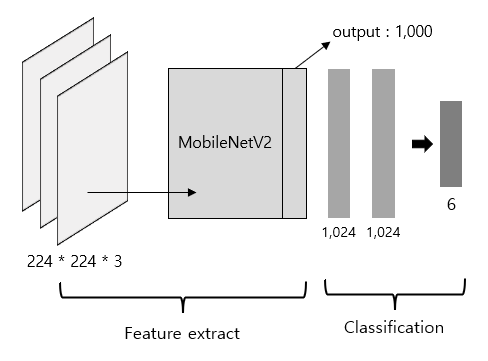
\includegraphics[width=6cm]{ENG/image-baseline.png} % Second figure file
        \caption{Image baseline}
        \label{fig.2}
        
    \end{minipage}\hfill
    \begin{minipage}{0.48\textwidth}
        \centering
        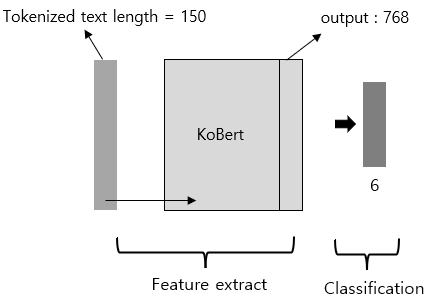
\includegraphics[width=6cm]{ENG/text-baseline.png} % First figure file
        \caption{Article text baseline}
        \label{fig.3}
    \end{minipage}
\end{figure}
%

\textbf{feature fusion 기준선}

이미지-텍스트 멀티 모달의 결정력을 파악하기 위한 모형이다.
텍스트와 이미지를 각각 KoBERT와 MobileNetV2에 입력한 후, output layer의 길이를 1024로 설정하여 두 도메인의 특성을 추출하였다.
이후, concatenate 방법을 적용하여 두 도메인의 특성을 길이가 2048인 벡터로 합친 뒤 길이가 각각 2048, 1024, 6인 classification dense layer을 이어주었다.
텍스트 데이터로 기사(Article)를 사용한 모형을 Article-Fusion, 주석(Annotation)을 사용한 모형을 Annotation-Fusion이라 부르기로 한다.

\begin{figure}[ht]
    \centering
    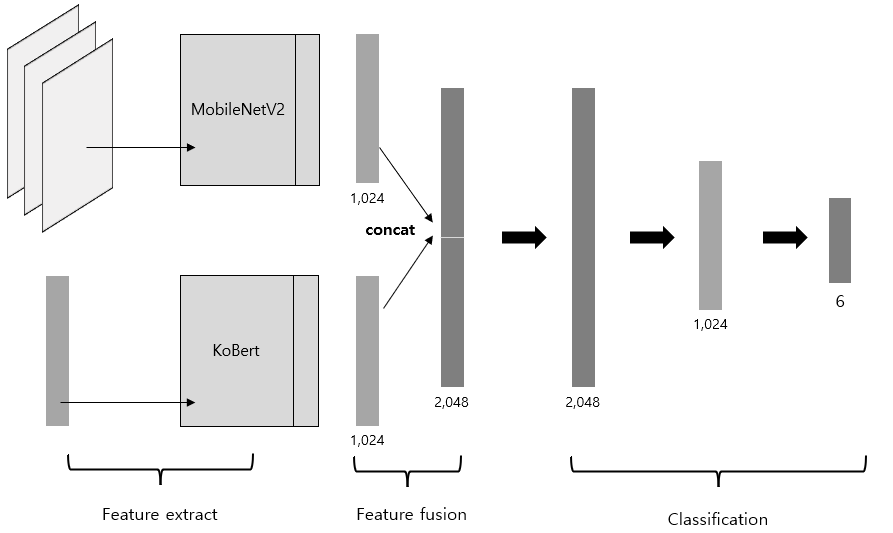
\includegraphics[width=8cm]{ENG/feature-fusion-baseline.png}
    \caption{Feature Fusion baseline}
    \label{fig.4}
\end{figure}

\textbf{앙상블 경쟁자 모형}

본 연구에서 제안하는 RoBaMF모형의 성능을 비교하기 위한 경쟁자 모형이다.
Article, Image, Article-Fusion 모형을 기본 분류기로 두고, K-fold 스태킹 앙상블 방법론을 적용한다. 메타 러너로는 XGBoost를 사용한다.
이 모형을 Competitor이라 부르기로 한다.



\textbf{RoBaMF 모형}

기사와 이미지의 고유한 특성과 함께, 이미지와 주석의 상호작용을 고려하는 모형이다.
Article, Image, Annotation-Fusion 모형을 기본 분류기로 두고, K-fold 스태킹 앙상블 방법론을 적용한다. 메타 러너로는 XGBoost를 사용한다.
이 모형을 RoBaMF라 부르기로 한다.



\textbf{K-fold 교차검증}

각 기준선 모형의 하이퍼 파라미터를 선정하기 위해, K-fold 교차검증을 적용하였다.
각 폴드마다 훈련 데이터를 다시 5760개의 훈련 데이터와 1440개의 검증 데이터로 분할하여 모형을 학습하였으며, 다음에 설명할 K-fold stacking ensemble을 위하여 모형의 가중치 학습 결과를 저장하였다. 5개 폴드의 Accuracy를 평균내어 모형의 성능을 사전 평가하였다. (Cross-Validation Accuracy)
이후, 최적의 하이퍼 파라미터와 훈련 데이터로 모형을 학습시킨 뒤, 시험 데이터를 예측하여 Accuracy를 계산하였다. (Test data Accuracy)
\textbf{K-fold 스태킹 앙상블}
Competitor, RoBaMF모형에는 교차검증을 도입한 스태킹 앙상블을 적용하였다.
6)의 모형 가중치 학습 결과를 불러와서, 각 폴드별로 검증 데이터와 시험 데이터에 대한 예측 결과를 산출하였다.
검증 데이터에 대한 예측 결과는 행 방향으로 이어 붙여서 MetaLearner의 훈련 데이터로 사용하였으며,
시험 데이터에 대한 예측 결과는 합산하여 MetaLearner의 시험 데이터로 사용하였다.
MetaLearner로는 XGBoost를 사용하였으며, 시험 데이터 예측 결과에 대한 Accuracy를 계산하였다.

\section{실험 결과}
\subsection{Baseline Models}
<이미지 기본 분류기의 저조한 결정력>
Image baseline : 모바일넷V2를 이용하여 특성을 추출한 이미지 기본 분류기는 40%에 미치지 못하는 교차검증 정분류율(Cross-Validation Accuracy)과 시험데이터 정분류율(Test data Prediction Accuracy)를 보여주었다.
이미지 기본 분류기의 저조한 결정력은 이미지 데이터의 모호함(ambiguity)에 기인한 것으로 추정된다.
예로, Fig.()의 대통령 사진은 politics 카테고리에 포함되어 있을 것으로 예상되나, 실제로는 life 카테고리에 포함되어 있다. -> life0.jpg 
또한, Fig.()와 같은 정부 상징을 비롯하여 브랜드 로고, 인물 사진들은 모든 카테고리에 분포하고 있어, 정확한 분류를 어렵게 만든다. -> science206.jpg

\begin{figure}[ht]
    \centering
    \begin{minipage}{0.48\textwidth}
        \centering
        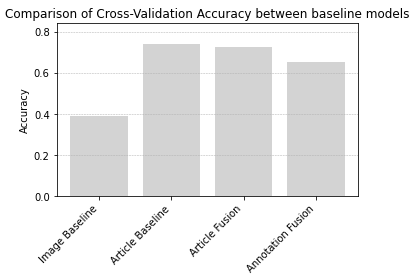
\includegraphics[width=7.5cm]{ENG/fig. 2.png} % First figure file
        \caption{K-fold CV accuracy of all baseline classifiers}
        \label{fig.5}
    \end{minipage}\hfill
    \begin{minipage}{0.48\textwidth}
        \centering
        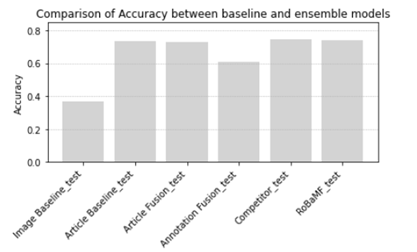
\includegraphics[width=7.5cm]{ENG/test-data-preds.png} % Second figure file
        \caption{Test data predictions accuracy.}
        \label{fig.6}
    \end{minipage}
\end{figure}


<Fusion 기본 분류기의 한계>
Article-Fusion baseline : 이미지와 Article에서 추출한  특성을 결합한 Article-Fusion 기본 분류기는 Article baseline보다 살짝 저조한 정분류율을 보여주었다.
이는 concatenate를 적용하였음에도 불구하고 두 모달리티의 특성을 결합하면서 각자가 가지고 있는 고유한 결정력이 저해되었거나, 멀티 모달에 맞는 옵티마이저나 하이퍼 파라미터를 잘 선택하지 않았기 때문이라고 생각된다.

Annotation-Fusion baseline : 이미지와 Annotation에서 추출한 특성을 결합한 Annotation-Fusion 기본 분류기는 Article-Fusion 기본 분류기보다 상당히 저조한 성능을 보여주었다.
대부분의 주석은 길이가 10단어 미만이므로, Article에 비해 담고 있는 정보가 제한적이기 때문에 KoBERT 특징 추출기가 결정력있는 특징을 출력하지 못한 것으로 보인다.

\begin{figure}[ht]
    \centering
    \begin{minipage}{0.48\textwidth}
        \centering
        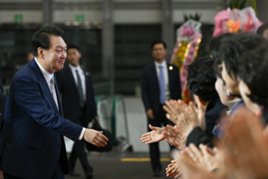
\includegraphics[width=6cm]{ENG/fig.4-1.png} % Second figure file
        \caption{A picture containing ambiguous imformation}
        \label{fig.7}
        
    \end{minipage}\hfill
    \begin{minipage}{0.48\textwidth}
        \centering
        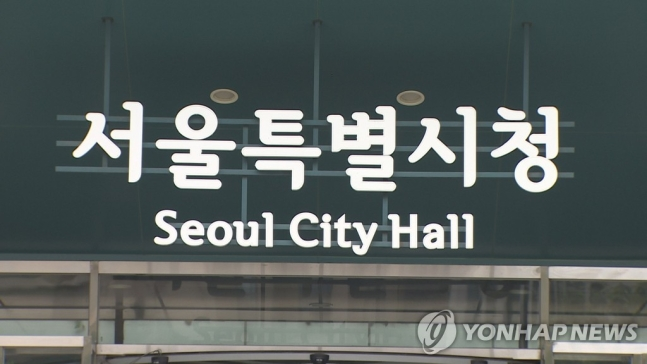
\includegraphics[width=6cm]{ENG/fig.4-2.jpg} % First figure file
        \caption{A picture containing ambiguous imformation 2}
        \label{fig.8}
    \end{minipage}
\end{figure}


\subsection{RoBaMF and Competitor}
RoBaMF와 Competitor 모형의 시험 데이터 정분류율은 Fig.()에서 확인할 수 있으며,
두 모형에서 각 baseline의 importance는 Fig.()에서 확인할 수 있다.

RoBaMF모형은 Article baseline과 동등하거나 미미하게 향상된 성능을 보였으며,
Competitor 모형은 Article baseline보다 약 1\%p 향상된 시험 데이터 정분류율을 보였다.
RoBaMF 모형이 더 많은 데이터를 사용하는데도 불구하고 성능이 저조한 것은,  Annotation-Fusion 기본 분류기와 Article-Fusion 기본 분류기의 결정력 차이에서 비롯한다.
이는 두 모형의 baseline importance가 뒷받침한다.
 RoBaMF 모형의 경우 Annotation-Fusion baseline이 평균적으로 11\%의 importance를 갖는데 반해, Competitor 모형의 경우 Article-Fusion baseline이 평균적으로 28\%의 importance를 갖는다.
추가적으로, 두 모형 모두 Article baseline의 importance가 다른 기본 분류기에 비해 압도적으로 높은 것을 고려해 볼 때, 이미지 기본 분류기와 Fusion 기본 분류기의 결정력이 충분하지 않음을 다시 한번 확인할 수 있었다.

\begin{table}[htbp]
\centering
\begin{minipage}[t]{0.45\textwidth}
\centering
\caption{Competitor}
\label{tab:competitor}
\begin{tabular}{@{}lllllll@{}}
\toprule
Condition       & \multicolumn{1}{c|}{ACC} & \multicolumn{3}{c}{Importance} \\
             & Value      & Image      & Article      & Fusion     \\
\midrule
Condition 1   & 0.745         & 0.003         & 0.699         & 0.297       \\
Condition 2   & 0.745         & 0.011         & 0.565         & 0.423       \\
Condition 3   & 0.750         & 0.001         & 0.751         & 0.247       \\
Condition 4   & 0.748         & 0.0008        & 0.819         & 0.179       \\
Condition 5   & 0.747         & 0.0002        & 0.751         & 0.248       \\
\bottomrule
\end{tabular}
\end{minipage}
\hfill
\begin{minipage}[t]{0.45\textwidth}
\centering
\caption{RoBaMF}
\label{tab:robamf}
\begin{tabular}{@{}lllllll@{}}
\toprule
Condition       & \multicolumn{1}{c|}{ACC} & \multicolumn{3}{c}{Importance} \\
             & Value      & Image      & Article      & Fusion     \\
\midrule
Condition 1   & 0.740         & 0.001         & 0.884         & 0.113       \\
Condition 2   & 0.738         & 0.010         & 0.780         & 0.209       \\
Condition 3   & 0.739         & 0              & 0.913         & 0.087       \\
Condition 4   & 0.739         & 0.0005        & 0.976         & 0.023       \\
Condition 5   & 0.739         & 0.0002        & 0.876         & 0.123       \\
\bottomrule
\end{tabular}
\end{minipage}
\end{table}


\begin{figure}[ht]
    \centering
    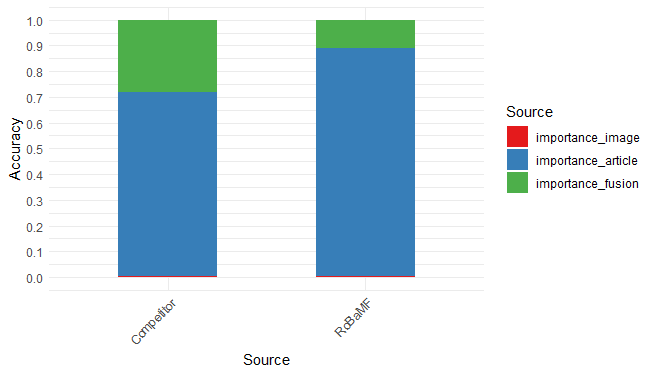
\includegraphics[width=8cm]{ENG/importance.png}
    \caption{Importance}
    \label{fig.last}
\end{figure}


\begin{table}[htbp]
\centering
\caption{XGBoost : Hyper parameters}
\label{your-label}
\begin{tabular}{@{}lllllll@{}}
\toprule
Conditon     & \multicolumn{2}{c}{Hyper parameter} \\
             & n      & lr      & lambda      & max-depth     \\
Condition 1   & 50         & 0.05         & 100         & 4        \\
Condition 2   & 500         & 0.05         & 500         & 5       \\
Condition 3   & 100         & 0.01         & 100         & 3       \\
Condition 4   & 100         & 0.001        & 100         & 4       \\
Condition 5   & 200         & 0.01        & 1000         & 5       \\
\bottomrule
\end{tabular}
\end{table}

\section{결론}
이미지 기본 분류기는 데이터의 모호함으로 인해 다른 분류기에 비해 낮은 정분류율을 보였다. Fusion 기본 분류기들은 특징 결합 (Feature concatenation)에 의한 결정력 저해로 인하여 Article 기본 분류기에 비해 낮은 정분류율을 보였으며, 특히 Annotation Fusion 기본 분류기는 주석의 제한적인 정보에 의해 더 낮은 성능을 보였다.
RoBaMF 모형은 Competitor 모형에 비해 더 많은 데이터를 사용하였지만, Fusion 기본 분류기의 결정력 차이에 의해 더 낮은 성능을 보였다.
향후 연구에서는 뉴스 데이터에서 두 모달리티의 고유한 결정력을 저해하지 않고 특징을 융합할 수 있는 방법을 고려해야 한다. 또한, kluebert와 같이 뉴스에 특화된 사전 학습을 거친다면, 주석의 제한적인 정보로 인한 결정력 저해를 극복할 수 있는지도 연구해야 한다.


이미지 기본 분류기는 모호한 이미지 데이터로 인해 낮은 분류율을 보였다. 반면 이미지와 기사 또는 주석을 결합한 Fusion Baseline들은 개별 모달리티의 결정력이 저하되고 특히 정보가 제한적인 Annotation Fusion 분류기는 더 낮은 성능을 보였다. RoBaMF와 Competitor 모델은  Article Baseline 분류기에 비해 약간의 성능 차이를 보였으나, modality gap 과 데이터의 모호성으로 인해 결정력이 제한적이었다. 이러한 결과를 바탕으로 향후 연구에서는 모달리티 간 통합을 개선하고, 다양한 데이터 소스의 결정력을 극대화 하는 방향의로서의 개선이 필요하다.








\bibliography{ref}
\bibliographystyle{plain}

%%%%%%%%%%%%%%%%%%%%%%%%%%%%%%%%%%%%%%%%%%%%%%%%%%%%%%%%%%%%
\end{document}
